\section{Properties of category scores}
This section illustrates several properties of the \CA\
scores through calculation and visualization.

\subsection{Optimal category scores}\label{sec:scores}
The singular values shown in \outref{out:corresp3.1} are the \(\lambda_i\), in Eqn. \eqref{eq:cadij}.  They are also the
(canonical) correlations between the optimally scaled categories.
Thus, if the \pname{DIM1} scores for hair color and eye color are assigned to
the 592 observations in the table, the correlation of these variables
would be 0.4569 --- the largest possible correlation for \emph{any}
assignment of scores.
The \pname{DIM2} scores give a second, orthogonal scaling
of these two categorical variables, whose correlation would be
0.1491.

In this sense, CA scores provide an optimal way of transforming
categorical water into quantitative wine,  hence the name ``optimal
scaling''.

We can illustrate this numerically and visually
as follows. If the row scores on dimension 1 are
in the $r \times 1$ vector $\vec{x}_1$ and the column scores are in the
$c \times 1$ vector $\vec{y}_1$, then these scores can be expanded to
conform with the $r \times c$ table by forming the appropriate outer
product with a unit vector:
\begin{equation*}
 \mat{X}_1 = \vec{x}_1 \: \vec{1}\trans
 \qquad \mbox{and} \qquad
 \mat{Y}_1 = \vec{1} \: \vec{y}_1\trans
 \period
\end{equation*}

The program below uses \IML\ to perform this operation on the \pname{COORD}
\Dset\ and then merges these scores with a reshaped copy of the
\pname{haireye} data.
The resulting \Dset\ is shown in \outref{out:cascores.1}.

The \CA\ scores then serve to quantify the hair color and eye color
categories producing the maximal possible correlations of $(X1, Y1)$ and
$(X2, Y2)$, while all other pairs are uncorrelated.
These correlations are shown in \outref{out:cascores.2}.
A plot of the optimal scores, using cell frequencies as weights
(\figref{fig:cascores}) is developed in the next subsection.
%% input: /users/faculty/friendly/sasuser/catdata/cascores.sas
%% last modified: 29-Jul-98 15:28
\begin{listing}
*-- Attach X, Y values to eye color, hair color and reshape;
proc iml;
   use coord;
   read all var\{dim1 dim2\} where (_type_='VAR') into var[r=eye]; hair=eye;
   read all var\{dim1 dim2\} where (_type_='OBS') into obs[r=eye];
   
   r = nrow(obs);
   c = nrow(var);
   x1 = obs[,1] * j(1, c);
   x2 = obs[,2] * j(1, c);
   y1 = j(r,1)  * t(var[,1]);
   y2 = j(r,1)  * t(var[,2]);
   
   hair = repeat( hair, r, 1);
   eye  = shape(repeat( eye, 1,c),r*c, 1);

   create scores var\{eye hair x1 y1 x2 y2\};
   append;
   quit;

*-- Reshape data to frequency form and merge with scores;
proc transpose data=haireye out=haireye2;
   var BLACK BROWN RED BLOND;
   by eye notsorted;

data haireye2;
   set haireye2;
   rename _name_=hair col1=count;

data scores;
   merge haireye2 scores;

proc print data=scores;
   format x1 x2 y1 y2 7.4;
   id eye hair;

*-- Correlations of scores = singular values;
proc corr data=scores nosimple;
   freq count;
   var x1 x2;
   with y1 y2;   

\end{listing}


\begin{Output}[htb]
\caption{Hair-eye data, DIM1, DIM2 scores assigned to hair-eye categories}\label{out:cascores.1}
\small
\verbatiminput{ch5/out/cascores.1}
\end{Output}
\ixd{hair-eye color}

\begin{Output}[htb]
\caption{Hair-eye data, correlations between X1, X2 and Y1 Y2}\label{out:cascores.2}
\small
\verbatiminput{ch5/out/cascores.2}
\end{Output}
\ixd{hair-eye color}

\subsection{Simultaneous linear regressions}
The correlations among the \CA\ scores have yet another interpretation which gave
rise to the first algebraic derivation of the technique
\citep{Hirschfeld:35} and which today provides an important concept in the
\citet{Gifi:90} system of homogeneity analysis.

Consider an arbitrary assignment of scores $X1$ ($Y1$) to the hair color
(eye color) categories, for example $X1$ ($Y1$) = 1, 2, 3, 4 for the
categories in alphabetical order.
Instead of plotting these scores along a dimension as in \figref{fig:corresp3}, we plot $Y1$ against $X1$ for all $n = 592$
cases and show the frequency at each discrete point by the area of
a bubble symbol, as in \figref{fig:cascore0}.

\begin{figure}[htb]
  \centering
  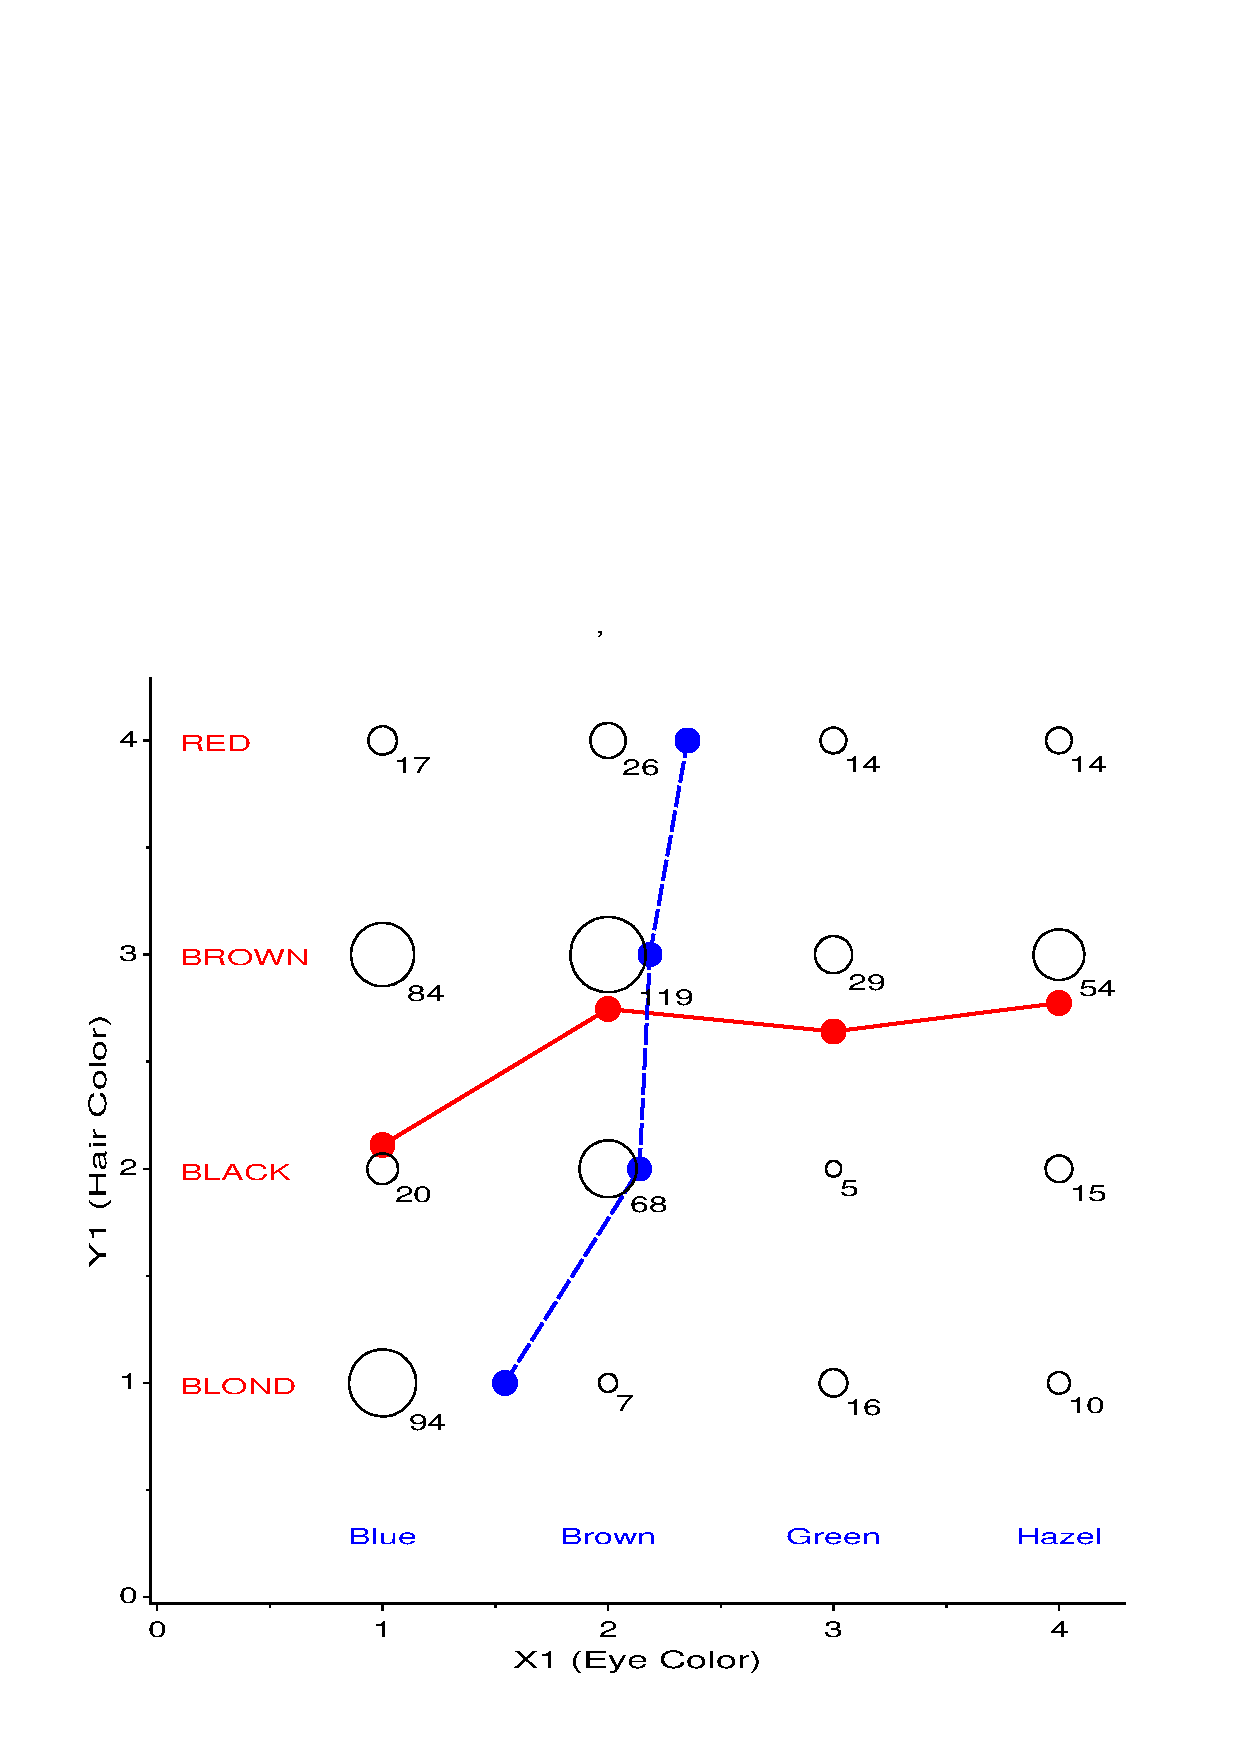
\includegraphics[scale=.6,clip]{ch5/fig/cascore0}
  \caption[Plot of arbitrary scores for the row and column categories]{Plot of arbitrary scores for the row and column categories.
The bubble symbols and numbers show the frequency at each point.
The red points (solid line) show the means of $Y1\given X1$; blue points (dashed line) show the means of $X1\given Y1$.}\label{fig:cascore0}
\end{figure}

If we carried out a least squares regression of  $Y1$ on $X1$,
this would be equivalent to finding the weighted mean of  $Y1$ for each value of $X1$ and fitting a straight line to these means.
Similarly, we could fit a regression of $X1$ on $Y1$,  which would be
determined by the weighted means of $X1$ for each $Y1$.
For the arbitrary scores, the conditional means of $Y1\given X1$
have a nonlinear relation to $X1$, and the same is true for the
inverse regression of $X1\given Y1$, as we see in \figref{fig:cascore0}.
The question posed by \citet{Hirschfeld:35} was this:
Can we find scores $\vec{a}$ and $\vec{b}$ for the row and column
variables such that \emph{both} regressions are linear?

The answer is ``Yes!''; indeed there is one solution for each pair of
\CA\ scores, $\vec{a}_i$ and $\vec{b}_i$, associated with the singular value $\lambda_i$.
For a given set of scores, $\vec{a}_i$ and $\vec{b}_i$, the weighted means
of the columns are
\(\mat{D}_c^{-1} \mat{P} \trans \vec{a}_i \), and the linear regression on
$\vec{b}_i$ has intercept 0 and slope $\lambda_i$,
\begin{equation*}%\label{eq:calin1}
(\mat{D}_c^{-1} \mat{P} \trans) \vec{a}_i = \lambda_i \vec{b}_i
\end{equation*}
Similarly, the inverse regression on $\vec{a}_i$ has intercept 0 and slope $1/\lambda_i$
\begin{equation*}%\label{eq:calin2}
(\mat{D}_r^{-1} \mat{P}) \vec{b}_i = (1/\lambda_i) \vec{a}_i
\end{equation*}
The choice of the scores associated with the largest singular value,
$\lambda_1$, makes the slope (equivalently, the correlation) of the
regression of $Y1$ on $X1$ as large as possible.
Moreover, this choice makes the angle between the two regression lines
as small as possible, i.e., the regressions are most collinear
\citep{Greenacre:84}.
So, instead of complex, nonlinear relations between the scaled
hair color and eye color variables using arbitrary scores (\figref{fig:cascore0}),
we arrive at simple, linear relations by use of a nonlinear
transformation of the arbitrary scores.

We can show these regressions for the first \CA\ dimension
in the following program steps, which continue from those
shown in \secref{sec:scores}.
Most of the program steps are concerned with finding the means
of $Y1\given X1$ and $X1\given Y1$, and annotating them on the
plot, together with the category labels and the regression line.
The plot with both regression lines is shown in \figref{fig:cascores}.
\begin{figure}[htb]
  \centering
  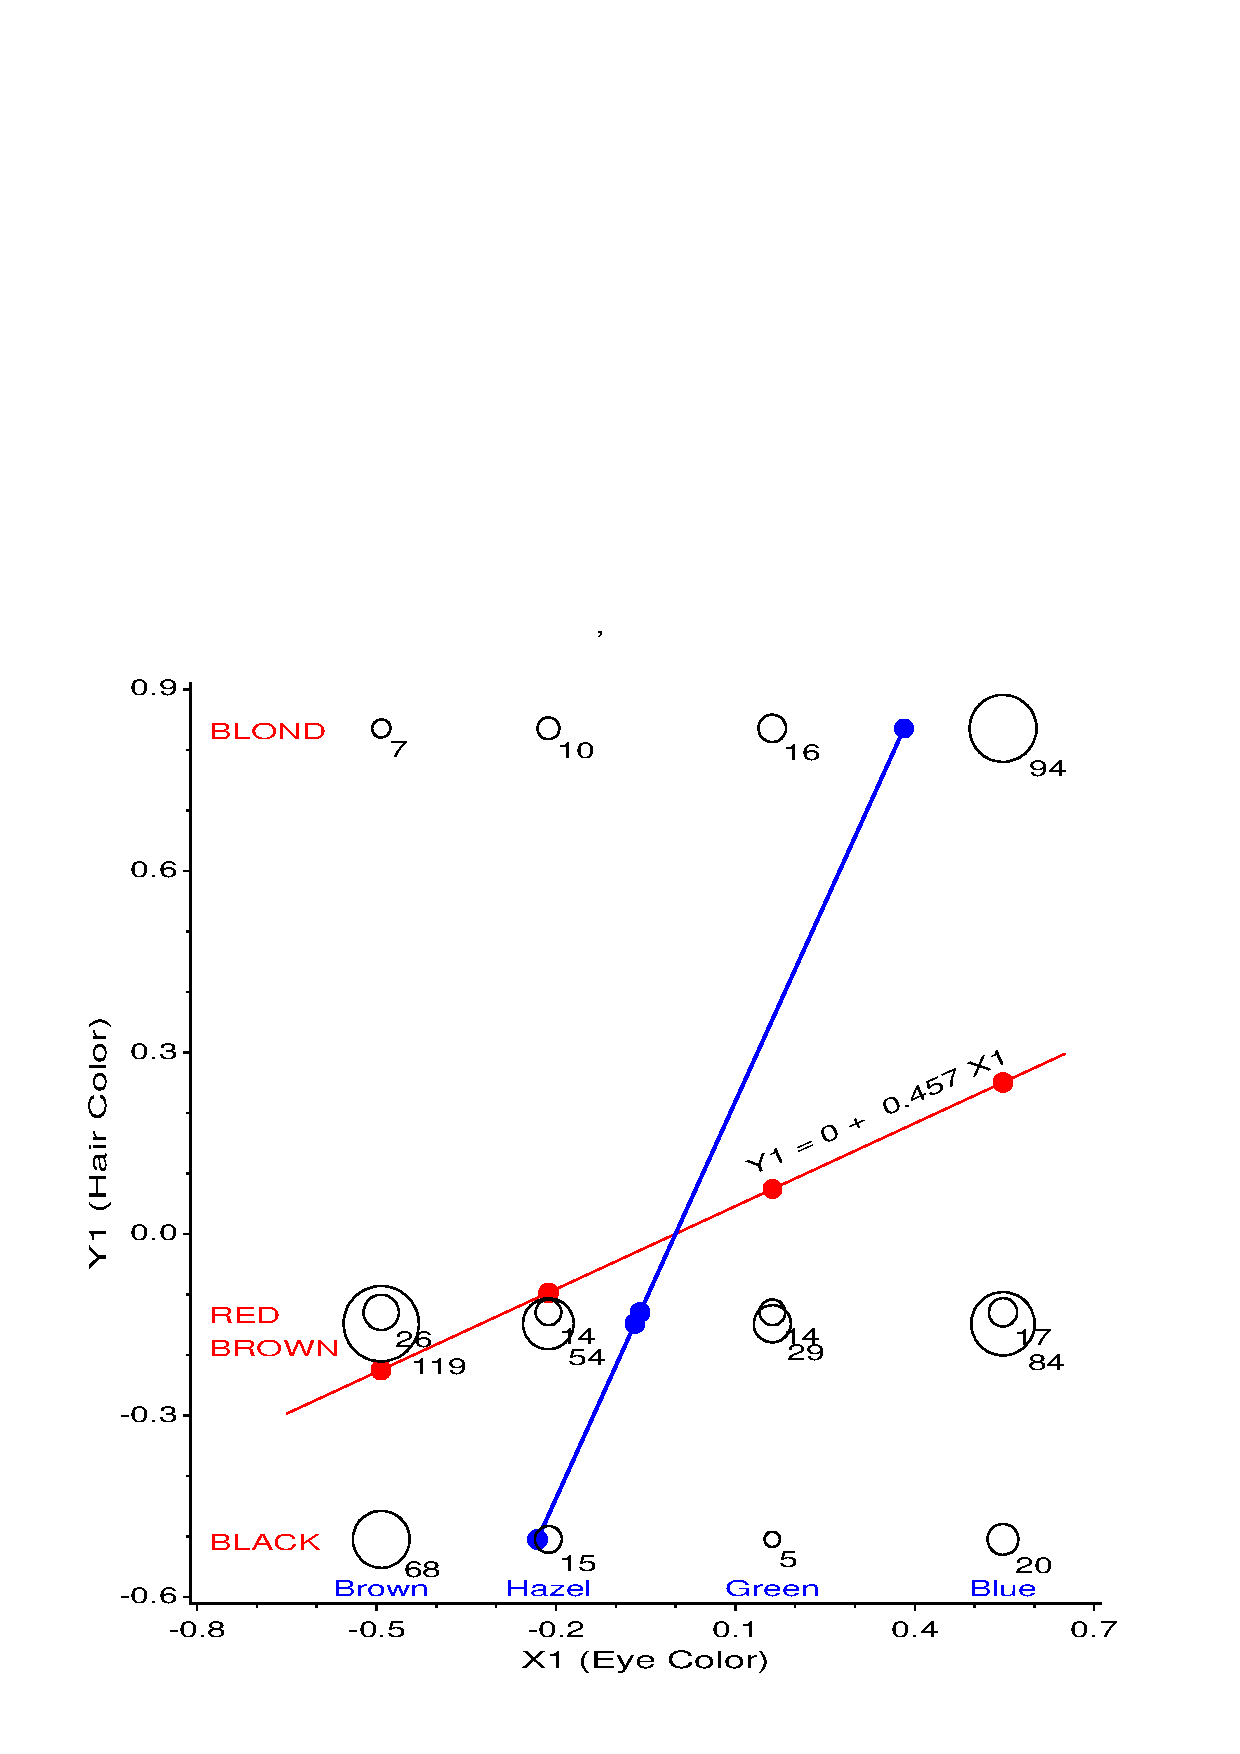
\includegraphics[scale=.6,clip]{ch5/fig/cascores}
  \caption[Simultaneous linear regressions of \CA\ scores for dimension 1]{Simultaneous linear regressions of \CA\ scores for dimension 1.  Using the optimal scores makes both regressions linear; choosing the scores associated with the largest singular value makes the two regressions most collinear.}\label{fig:cascores}
\end{figure}
%% input: /users/faculty/friendly/sasuser/catdata/cascores.sas
%% last modified: 04-Aug-98 13:31
\begin{listing}
*-- Annotate the row and column means;
proc means data=scores nway noprint;
   var y1;
   class x1;
   freq count;
   output out=ymeans mean=y1bar;
data ymeans;
   set ymeans;
   retain xsys  ysys '2' size 2;
   x = x1; y = y1bar;
   function = 'symbol'; text='dot'; color='red';  output;

proc means data=scores nway noprint;
   var x1;
   class y1;
   freq count;
   output out=xmeans mean=x1bar;
data xmeans;
   set xmeans;
   retain xsys  ysys '2' size 2 line 4;
   x = x1bar; y = y1;
   function = 'symbol'; text='dot'; color='blue';  output;
   if _n_=1 then function='move';
      else function='draw';
   output;

*-- Annotate the row and column labels;
data label1;
   set scores(keep=eye hair x1 y1);
   where eye='Brown';
   retain xsys ysys '2' color 'red    ' function 'label   ';
   if hair='BROWN' then position='9';
      else position='6';
   x = -.78; y = y1; text = hair;
data label2;
   set scores(keep=eye hair x1 y1);
   where hair='BLACK';
   retain xsys ysys '2' position '5' color 'blue' function 'label   ';
   x = x1; y = -.58; text = eye;

*-- Get slope and intercept of (weighted) regression line;
proc reg data=scores outest=parms noprint;
   model y1 = x1;
   weight count;

data line;
   set parms (keep=x1 intercep);
   drop x1 intercep;
   length text $20;
   
   *-- Draw (weighted) regression line;
   xsys='2'; ysys='2'; color='red   ';
   x=-0.65; y = intercep + x1 * x; function='MOVE    '; output;
   x= 0.65; y = intercep + x1 * x; function='DRAW    '; output;
   x= 0.35; y = intercep + x1 * x; function='LABEL   '; color='black';
   angle = atan(x1) * (45/atan(1)); position='2';
   text = 'Y1 = 0 + ' || put(x1,6.3) || ' X1';  output;
   
*-- Combine the annotate data sets;
data labels;
   length text $20;
   set label1 label2 line ymeans xmeans;

proc gplot data=scores;
   bubble y1 * x1 = count / 
      blabel bsize=8 bscale=area
      vaxis=axis1 haxis=axis2 hm=2 vm=2 anno=labels;
   axis1 order=(-.6 to .9 by .3) label=(h=1.8 a=90 'Y1 (Hair Color)');
   axis2 order=(-.8 to .7 by .3) label=(h=1.8      'X1 (Eye Color)');
   \end{listing}

Note that the slope of the line for $Y1\given X1$ in \figref{fig:cascores} is 0.457, the largest singular value and the largest canonical correlation.
If we were to repeat these steps using the \CA\ scores $X2$ and $Y2$
on dimension 2, we would find another pair of linear regressions, with
a slope of 0.149 for $Y2\given X2$, the second singular value.
